\documentclass[a4paper,11pt]{jreport}

%%\usepackage[dvipdfmx,bookmarks=true,bookmarksnumbered=true,bookmarkstype=toc]{hyperref} \usepackage{pxjahyper}
%%\usepackage{ulem}
\usepackage[dvipdfmx]{graphicx} % for \includegraphics[width=3cm]{sample.pdf}
\usepackage{times} % use Times Font instead of Computer Modern
\usepackage{ulem}

\setcounter{tocdepth}{3}
\setcounter{page}{-1}

\setlength{\oddsidemargin}{0.1in}
\setlength{\evensidemargin}{0.1in}
\setlength{\topmargin}{0in}
\setlength{\textwidth}{6in}
%\setlength{\textheight}{10.1in}
\setlength{\parskip}{0em}
\setlength{\topsep}{0em}

%% タイトル生成用パッケージ(重要)
\usepackage{coins-jp}

%% タイトル
\title{差分プライバシー保証のための \\ 汎用プログラミングフレームワークの設計}
%% 著者
\author{}
%% 指導教員
\advisor{}

%% 年度と主専攻名
\fiscalyear{2022}
\majorfield{情報システム主専攻}

\begin{document}
\maketitle
\thispagestyle{empty}
\newpage

\thispagestyle{empty}
\vspace*{20pt plus 1fil}
\parindent=1zw
\noindent
%%
%% 論文の要旨
%%
\begin{center}
{\Large \textbf 要旨}
\vspace{2cm}
\end{center}
現代において利用者の個人情報を収集し、多目的用途のために統計処理を行う。
しかし、安易に情報を外部の組織へ譲渡してしまうと漏洩や悪用の可能性がある。
個人情報を保護する手法は複数存在するが、その中に差分プライバシー技術が存在する。
これはデータの出力値に対してノイズを加えることで、出力値のみを知っている場合に他の情報と差分を組み合わせても元の生データを逆算できないように加工する技術である。
従来の研究ではあらかじめ指定された演算をして差分プライバシーを用いて出力するものがあるが、計算の柔軟性やプログラミング言語の選択肢が限られているという問題があった。
本研究では、差分プライバシー技術とWebAssemblyによるサンドボックス技術を組み合わせた。
WebAssembly技術はプログラミング言語に依存しないバイナリ形式のプログラムを実行するための技術である。
プログラムはWebAssemblyのランタイム内部でのみ実行されるためサンドボックスとしても利用できる。
これにより任意の言語で書かれた任意のプロセスが自由にフィルタリング・データ加工・計算を行えるが、プロセスの外部への勝手なデータ漏洩を防止することが可能となった。
データを出力する際も生のデータの出力をシステムコールレベルで禁止し、あくまで差分プライバシーを適用した統計値のみを出力できるようにする。
また差分プライバシーを適用した出力をするために独自システムコールの実装をした。
これにより個人情報の漏洩を抑えつつ、今までより柔軟な計算を用いた統計処理が、WebAssemblyに対応した任意の言語で可能となる。
差分プライバシーのノイズ計算自体も、ランタイムのソースコード自体を変更せずに別プロセスとして独立させ、拡張機能として自由に選択できるようにした。
これらの提案をもとに実際にフレームワークを開発した。
フレームワークを用いることで、複数のプログラミング言語で大幅な修正を必要なく簡単な差分プライバシー導入が可能となった。
その後実際に統計処理プログラムを実行することで、差分プライバシー技術の有効性を検証した。実行時間性能のベンチマークも行いオーバーヘッドの評価した。

%%%%%
\par
\vspace{0pt plus 1fil}
\newpage

\pagenumbering{roman} % I, II, III, IV
\tableofcontents
\listoffigures
%\listoftables

\pagebreak \setcounter{page}{1}
\pagenumbering{arabic} % 1,2,3

\chapter{序論}

情報化が進んだ現代で、個人情報を含むデータへのプライバシー保護が重要になっている。
しかし、アプリケーションの脆弱性を突いた攻撃や情報漏洩を目的としたマルウェアへの感染、
複数のデータベースを組み合わせ共通している列を見つけ出す、
匿名化していてもその情報の組み合わせを持つ人が1人しか居ないなど、様々な手法で$k$匿名性\cite{k-anon}が破れ個人情報は漏洩してしまう。

それらの対策として、差分プライバシー技術が存在する。
これは、データに特定個人が存在する場合としない場合の統計結果が区別できないようなノイズを載せる手法である。
これを用いて個人情報の漏洩を防止する。
ノイズの実現方法の例としては、ラプラス分布やガウシアン分布が挙げられる。
これによりノイズが載っていても”尤もらしい”データを出力できる。

しかし、既存の差分プライバシー技術は複雑な統計処理が困難という問題がある。
そのため本研究では、任意の演算を行い複雑な統計処理と差分プライバシーの両立を実現することが目的である。
この研究により、新たに複雑な統計処理が実現可能となる。

\chapter{研究背景と目的}

\section{現状と課題}

個人情報など単体では重要度の高いデータ列を利用して、統計値を取得し研究や産業へ活用できる。
具体的には、年齢・性別・病歴・位置情報などのデータから、商品の購買頻度や移動距離、関心のある広告などの情報を得ることが考えられる。
これらの個人情報は通常個人が利用するサービスや企業に蓄積されるが、その個人情報を別の企業・システムへ提供し利用する場合がある。
そういった場合に個人情報を信頼できない企業・システムへ直接提供してしまうと、提供先企業に悪意がある場合、また外部から不正アクセスを受けた際に
個人情報を含むデータの生の情報を含む列が漏洩してしまう可能性がある。
そういった場合に情報が漏れてしまっても個人情報を特定できないようにデータを加工して、
生ではないデータのみを共有する技術など、プライバシー保護をする技術が求められる。

既存の攻撃として、データベースの統計結果の差分からデータを逆算する手法がある。
例えばデータベースA(図\ref{fig:database-a})が存在する。
ここに新たなデータ列「Cさん」を追加した場合データベースAはデータベースA'(図\ref{fig:database-a2})に変化する
攻撃者は、両者の平均値とデータ個数のみを知っているとする。
この時、Cさんの年収を$x$と置き以下のような式を立てることができる。

(avg(A) * count(A) + x) / count(A') = avg(A')

実際に代入すると x = 700 となるため真のデータが逆算できてしまう。

\begin{figure}[htbp]
    \centering
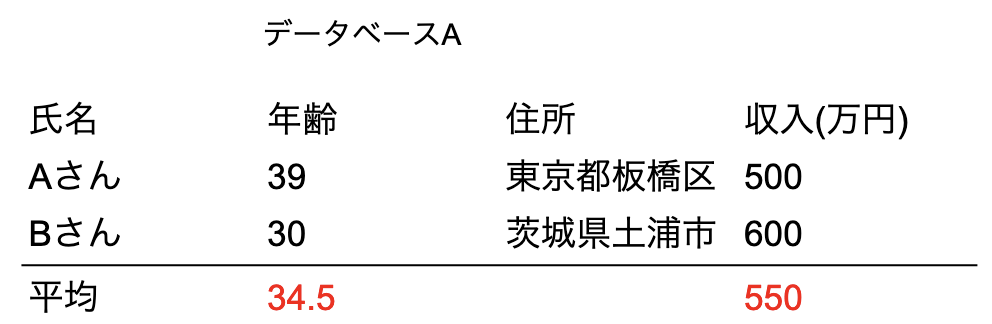
\includegraphics[height=50mm]{database-a.png}
    \caption{データベースA}
    \label{fig:database-a}
\end{figure}

\begin{figure}[htbp]
    \centering
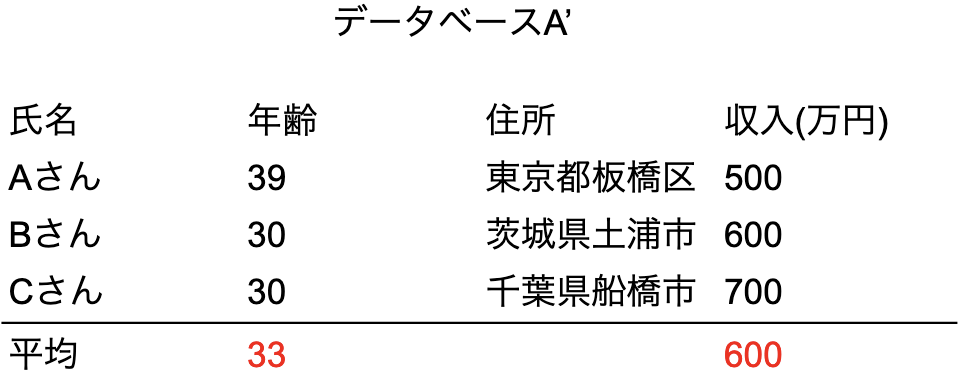
\includegraphics[height=50mm]{database-a2.png}
    \caption{データベースA'}
    \label{fig:database-a2}
\end{figure}

\section{差分プライバシー}
プライバシー保護の1つに差分プライバシー技術がある。\cite{dp}

\subsection{概要}
差分プライバシーの基本的な概念では、データベースに対して個人情報を新たに追加した際に、
追加前のデータベースから得られる統計情報と追加後のデータベースから得られる情報の差分から新しい個人情報を特定できないようにする。
その手法としてノイズを生成して付加する。

\subsection{ノイズ分布}
差分プライバシーの実現方法の1つとして、ラプラス分布やガウシアン分布を用いてノイズを付加する方法がある。
例えば合計値や平均値、最大値など統計値を計算する場合、まず通常通り計算する。同時に、それらの統計値に利用したベクトル列
から数値の範囲、ばらつきを取得する。
次に、ラプラス分布やガウシアン分布のように、中央がもっとも大きくなるような分布関数を選ぶ。この時分布関数の裾野の大きさを決定するために、
パラメーターとして先ほど取得した数値の範囲やばらつきを使用する。
この時、数値の範囲が大きすぎると統計値として有用でなくなってしまうため、あらかじめどれぐらいの確率で真の値が出現できるかの確率を設定する必要がある。
分布関数を決定したら、乱数の分布が分布関数にそうような乱数を生成する。
これは、例えば分布関数の逆関数の積分に一様乱数を代入することで実現できる。\cite{rand}

\subsection{差分プライバシーの適用}
最終的に計算結果の出力結果に対して、これらの乱数を差分として追加する。
こうして追加された差分は、人一人分の情報がデータベースの統計結果に対して与える影響を確率的に遷移させることになり、
結果として個人情報を逆算することを防ぐことができる。よってこれらの差分はもっともらしいノイズと言える。
以上の操作により統計結果から元のデータ列を逆算することが難しくなる。
もちろん差分プライバシーの計算自体は安全な領域で行う必要がある。

\section{関連研究}

\subsection{PipelineDP}

差分プライバシーを用いた既存研究では、Royce J Wilsonらによる先行研究\cite{dpsql}がある。
これは、差分プライバシーを適用した状態でApache Spark\cite{apache}などの分散データ処理を行うデータベースにアクセスするSQLの提案である。
この研究では、信用できないソフトウェアがSQLクライアントとして個人情報が含まれるデータベースにアクセスする。
データベースに対してクエリを投げると、事前に差分プライバシー適用済みで統計値を計算し、その結果のみがクライアントに返ってくる仕組みである。
この研究の成果としてGoogleの多言語差分プライバシーライブラリであるDifferential Privacy\cite{googledp}やOpenMindによるPipelineDP\cite{openmind}が開発された。
これはSQLの文法が実現できる範囲で統計を処理するソフトウェアの場合に有用である。

\subsection{Apple}

AppleはiPhoneのOSであるiOSにおいて、データの収集をする際に、差分プライバシーを活用している。\cite{apple}
ユーザーがよく使う絵文字や、Safariでよく電力を使用するドメイン、ユーザーが選択した予測変換のリストなどの
データベースをローカルに保持する。このデータベースからランダムに複数行を取り出したうえで
統計処理を行い、差分プライバシーを適用してからリモートのサーバーへ送信する。
サーバーは各クライアントから送信されたデータを収集し、さらなる統計処理を行う。

\begin{figure}[htbp]
    \centering
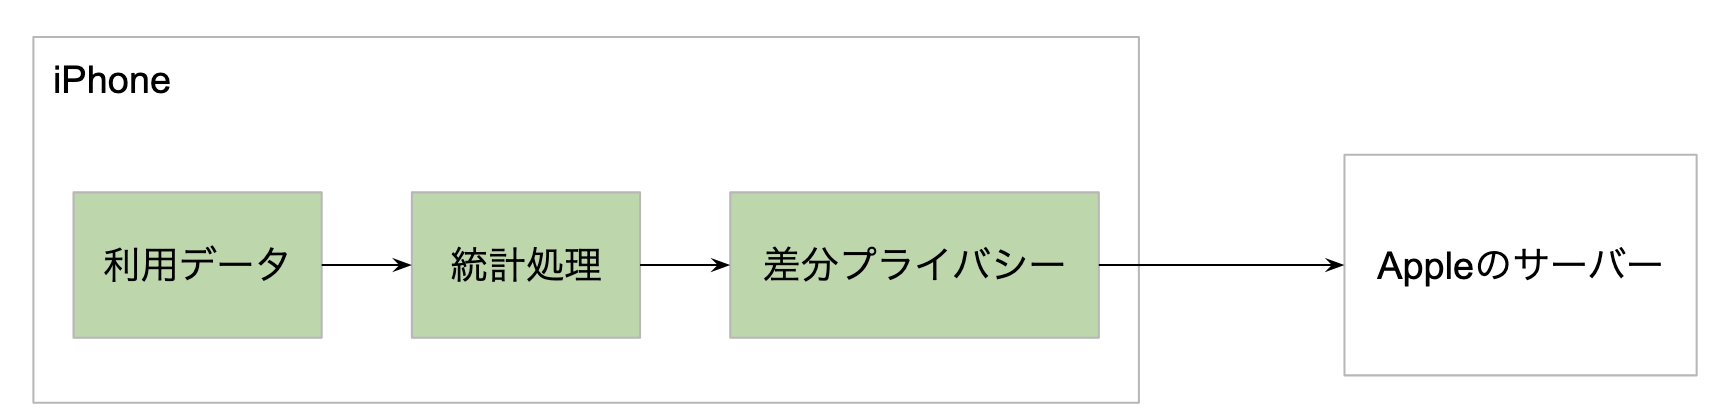
\includegraphics[height=20mm]{apple.png}
    \caption{Appleでのローカル差分プライバシーの活用}
    \label{fig:apple}
\end{figure}

\subsection{問題点}

一方これらの手法では、統計結果を前提に別の統計結果を実行したり、生の個人情報を直接計算に利用した複雑な統計処理などはできない。
またSQLの関係代数で表現できない演算は行えなかったり、できたとしてもクエリが複雑になってしまうといった問題がある。
そういった事例としては、2次元ではない多次元に対する平均や最頻値の処理、
データを元に機械学習をしてそのネットワークを出力する処理、
値を丸め込み代表値として扱うなど事前のフィルタリング処理がデータに必要な場合、
数値ではなくnビットの情報量(都道府県など)を扱いたい場合が挙げられる。

\section{要求項目}

以上の背景をもとに、今回提案するシステムで要求される項目を以下に示す。
\begin{itemize}
    \item SQLなどの関数型構文だけではなく、順序実行・条件分岐・繰り返しなど汎用的なプログラミングの構文を扱える
    \item 生の個人情報データには計算途中で直接アクセスできる
    \item プログラムが外部に情報を出力する際は、もっとも最後の統計値に差分プライバシーを適用した場合のみに限る
    \item プログラムの実行結果は、プログラムの実行前に差分プライバシーを適用した統計値を元に逆算できない
    \item 統計結果はプログラムではなく信頼できるソフトウェアによって計算される
\end{itemize}

\chapter{WebAssembly技術}

\section{概要}

本研究では実装にWebAssemblyを用いた。
WebAssembly技術は、Webブラウザ上で動作するプログラムをコンパイルするための仕様である。
技術の本体は言語仕様となっており、名前の通りアセンブリ言語によく似た構造である。
WebAssembly技術のメリットは、コンパイラのターゲットにWebAssemblyが対応すればその言語をWebAssemblyが動作するどの環境でも実行できる点である。
この時環境のことをランタイムと呼び、WebAssemblyのランタイムはWebブラウザに組み込まれている。
このランタイムはWebAssemblyのバイナリを読み込み、実行するための仮想マシンとして機能する。
そのためサンドボックス技術のように扱うことができる。
デメリットとしては通常のネイティブ環境で動作するバイナリとは別に、ソースコードをWebAssemblyに再コンパイルする必要がある点や、
実行時にランタイムの層が追加されることでパフォーマンスが低下する点が挙げられる。
他にも、WebAssemblyはバイナリフォーマットであるため、ソースコードを読むことができない点や、
さまざまな言語のコンパイラでサポートが必要になる点などが挙げられる。
また一番の問題として、WebAssemblyはWebブラウザ上で動作するプログラムをコンパイルするための仕様であるため、システムコール仕様に沿っていない動作をする場合は
その機能をランタイム側で実装する必要がある。

\section{Web Assembly System Interface}

Web Assembly System Interface(以下WASI)\cite{wasi}は、通常ブラウザ上で動作するWebAssemblyプログラムに対して、サーバーやデスクトップ環境など
ブラウザ以外の環境で動作する場合に、必要なシステムコールを提供するための仕様である。
例えばファイル読み書きやソケット通信、スレッドの生成、割り込み処理などがある。
ブラウザで動作する場合にこれらはブラウザやランタイム側が提供するため不必要だが、単体のアプリケーションとして動作する場合には必須となる。
WASIは旧来のPOSIXのシステムコールを基盤としつつ、サンドボックスのために不必要な機能を削除し、またWebAssemblyのデータ構造仕様に合わせて
作られたため、POSIXのシステムコールとは互換性がない。
そのため、既存のC言語のプログラムをWebAssemblyにコンパイルする場合は、POSIXのシステムコールをWASIのシステムコールに変換する必要がある。
通常これらの動作はコンパイラによって行われるが、言語使用によってはブラウザ上で動作するWebAseembly形式のバイナリを生成することのみに
対応している場合があり、プログラミング言語全てにおいて対応が万全とはいえない。

WASIに対応するWebAssemblyランタイムとして、WasmTime\cite{wasmtime}やWasmer\cite{wasmer}などが挙げられる。これらは、WASIの使用に沿ったWebAssemblyバイナリを実行し
システムコールが呼ばれるとランタイムとしてその処理を行う。WebAssemblyがユーザー空間だとすると、対してカーネル空間のような役割を果たす。
WasmTimeやWasmerは、WASIの仕様に沿ったシステムコールを実装しているため、自分で全てのシステムコールを実装したりバイナリ解析をせずとも、
これらのランタイムを使用し拡張する形式で開発することで、新しい機能の追加のみに注力してランタイムを開発できる。

\section{WASIの策定状況}

WASI自体は未だ新しい仕様であり、現在のところは仕様の策定段階である。2022年現在ではスナップショットバージョンとして公開されている
仕様があり本研究ではそれに対応した。
スナップショットバージョンでは、基本的なシステムコール、例えば標準出力やファイルアクセス、環境変数などが定義されている。
その一方、スレッドやメモリマッピング、ネットワークアクセスなどの機能はまだ策定途中であり、頻繁に仕様が変更される。
そのため言語のコンパイラによっては追従していない場合もある。
こういった問題に対応するため、WASIではシステムコール名のみを策定してその実装をダミーとして定義したり\cite{wasi-pr-thread}、
既存のシステムコールを組み合わせて下位互換のシステムコールを再現する形\cite{wasi-issue-thread}で仕様を途中まで固めている。
その他の対応策として、libcに概要するような標準ライブラリwasi-libcをC言語など一般的なプログラミング言語に提供し、
プログラムはそのライブラリを呼び出す形でシステムコールを使うという手段も提案されている。
システムコールを直接呼び出す行為はプログラムにWebAssemblyに対する直接的な知識や特別なサポートを要求するため、
さまざまな環境で同じソースコードを動作させようと考えた場合にはこの方法が必須である。

\chapter{提案手法}

\begin{figure}[htbp]
    \centering
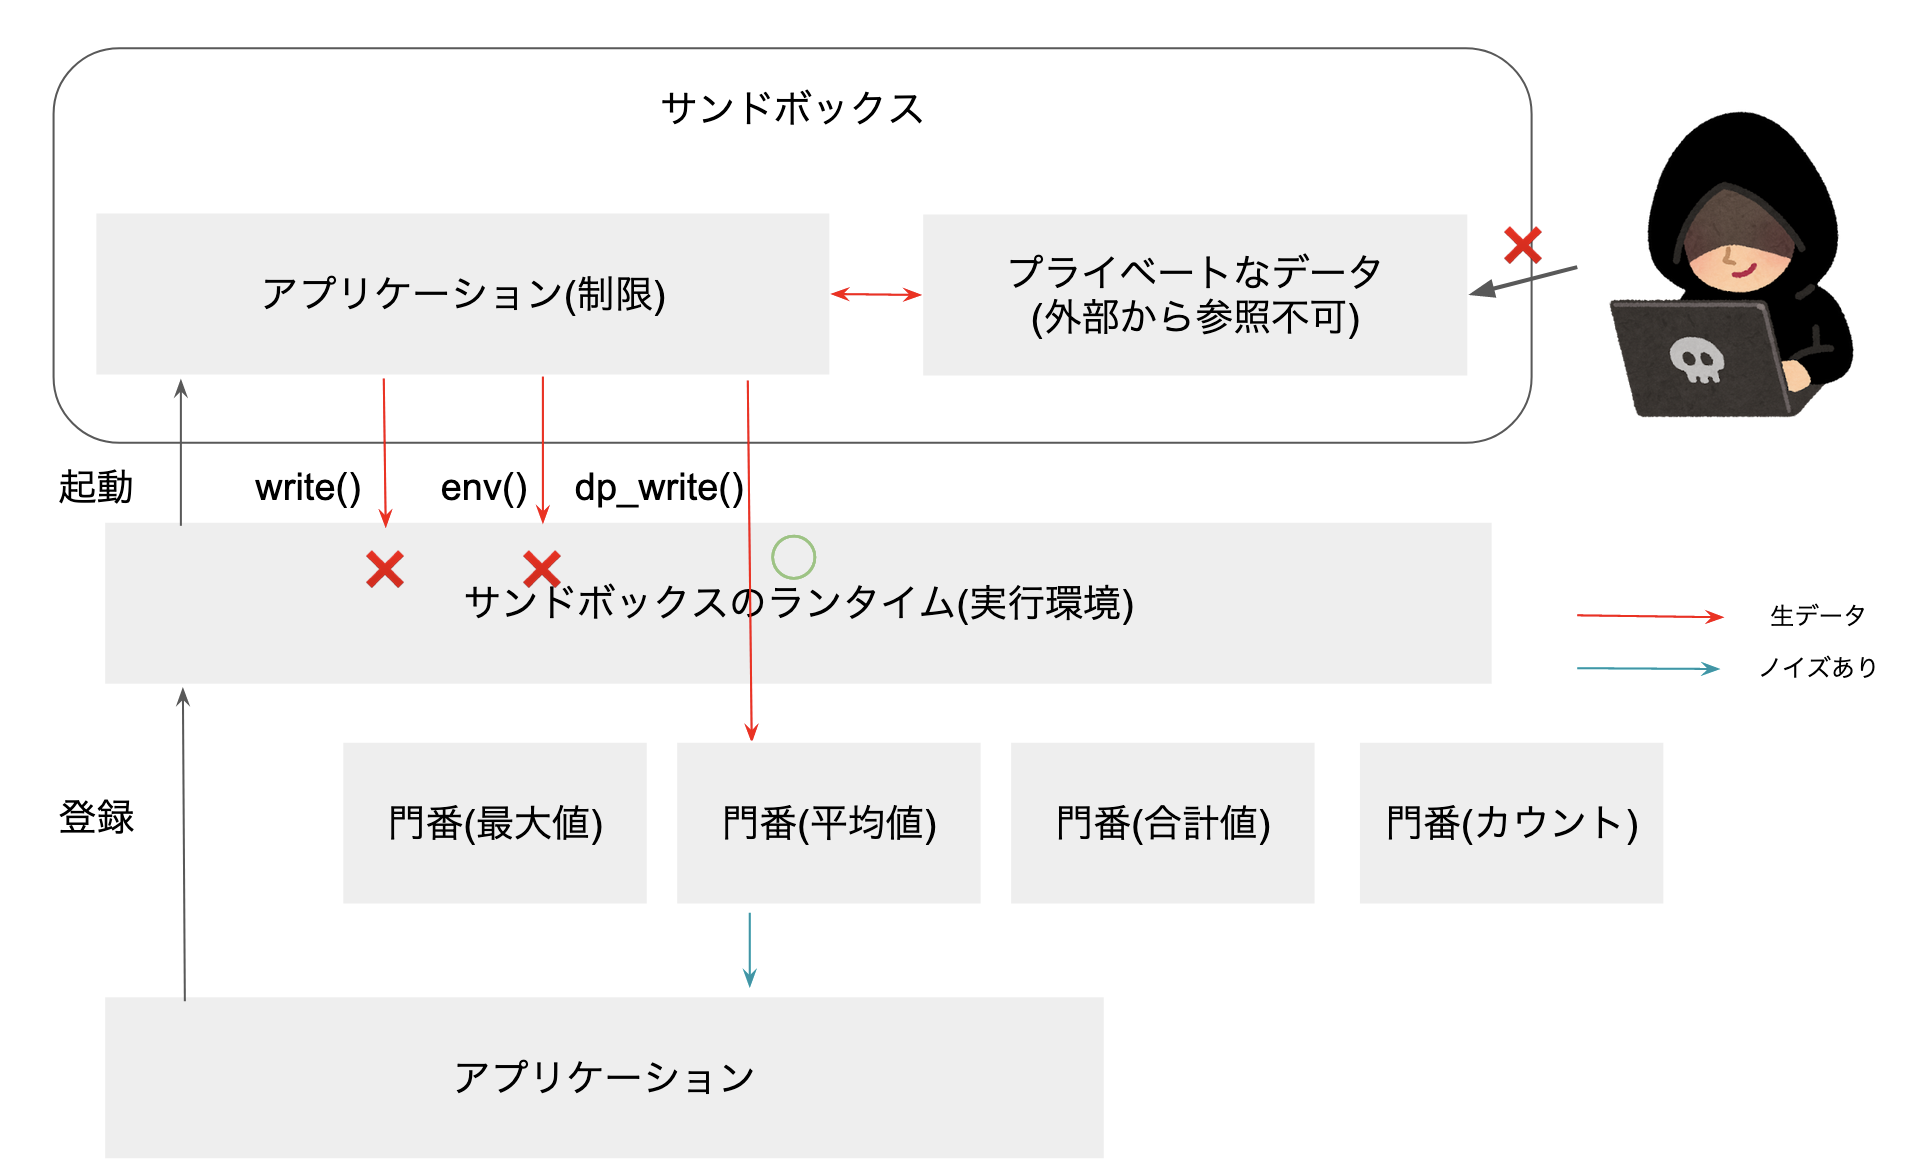
\includegraphics[height=80mm]{architecture2.png}
    \caption{フレームワークのアーキテクチャ}
    \label{fig:architecture}
\end{figure}

\section{システム構成}

本研究で提案するシステムの全体像を図\ref{fig:architecture}に示す。
本システムは、プログラムの実行をサンドボックス型のフレームワークで行うことで、統計値に対して差分プライバシーを適用し、統計値から元の値を逆算できないようにしている。
本システムの構成は以下の通りである。

\subsection{サンドボックス}

この研究では、任意の仮想的な計算機(=サンドボックス)を用いて、サンドボックス型のフレームワークを開発・評価することで、任意のプログラムの実行を可能にし幅広い統計処理を実現する。
今回使用するサンドボックスは、前述するようにWebAssembly技術を利用している。
任意の言語で書かれたプログラムを、コンパイラでWebAssembly形式にコンパイルし独自のランタイムで実行する。
WebAssemblyはWebブラウザ向けに開発された中間言語で、
あらかじめさまざまな言語からコンパイルされたバイナリ形式のファイルをランタイムが動くさまざまな環境で動作させることができる技術である。
本フレームワークでは、サンドボックスを利用することで、
内部では差分プライバシーに対応した出力を行えるシステムコールのみ許可し、
通常のファイル読み書きやネットワーク接続の禁止や条件付きの許可をする。
プログラムからプライバシーを守りつつ内部では統計処理を自由に行うことができる。(図\ref{fig:architecture})
サンドボックスはシステムコールのブラックリスト機能を持っている。
これにより、あらかじめプライバシー保護のために禁止しておきたい命令を指定することで、標準出力やソケット通信を防ぐことができる。
外部出力が可能となるようなシステムコールは、ブラックリストで無効化され、
例え実行しても何も起こらずにシステムコールが正常終了する。

\subsection{独自システムコール}

本システムでは、差分プライバシーに対応したシステムコールとして privacy_out_vec を追加した。
既存ランタイムであるWasmerのライブラリを用いて、新たな名前空間に差分プライバシー専用のシステムコールを追加する形で実装した。
これは引数として差分プライバシーを適用するパラメーターと、出力したい統計値の元となるベクトル、統計計算の種類を引数として受け取る。
ランタイムはこのシステムコールが実行されると門番に対してその引数を渡すことで、実際に差分プライバシーを適用した統計計算を行う。
門番は、差分プライバシーを適用した統計値をサンドボックスに返すことで、プログラムの実行を継続する。

\subsection{ライブラリ}

本フレームワークの一部として各言語用にライブラリ・ラッパーを提供する。
これは、どの言語からでも同じシステムコールを用いて差分プライバシーの実行をランタイムに命令できる。
差分プライバシーを用いて出力する際も、出力する関数を置き換えるだけなど、プログラムの変更が必要最低限に抑えられる。

\subsection{門番}

サンドボックスが出力した生のデータは、信頼できる差分プライバシー計算機(=門番)が統計処理を行う。
また出力形式としては、平均値や中央値、標準偏差や信頼区間、分散や総和を想定している。
門番はあらかじめランタイムとは別のプログラムとして独立し、ランタイムからはどの門番も統一されたインターフェースから呼び出しができる。
門番は受け取ったデータから指定された統計処理を行い、同時にデータのばらつきから孵化するべきノイズ分布関数の大きさを決定する。
その後、分布に沿うように生成したノイズを統計結果に加算し、出力する。
詳しくはノイズ処理の節を参照。

\section{ノイズ処理}
本研究では、差分プライバシー技術を適用しながらも複雑な統計処理を実現するために、新たな手法を提案する。
それには、実現したい統計処理のデータ幅や偏差に適したノイズを生成し、統計結果が区別できない程度にだけノイズを加える。

\subsection{ノイズの生成}

出力する値にノイズを乗せる手法として、差分プライバシー技術を用いる。
サンドボックス内部のプログラムは、統計値に対して出力したい値、例えば平均値や合計値を直接計算せずに、門番に対してベクトル値をその計算種類を与える。
門番は、そのベクトル値から実際の合計値・平均値を計算する。その後ベクトル値のばらつきから偏差を求めて、ガウス分布にそう乱数を生成し、それを結果に対して加算する。
これにより、統計値にはガウス分布に従うノイズが加算される。
分布関数の裾野の大きさを、あらかじめ設定することで、ノイズの乗った値から真の値を見つける難易度を設定できる。

\subsection{ラプラス分布のパラメーター}

変化前のデータベースAと変化後のデータベースA'がある。
それぞれノイズを適用した場合のAの確率分布とA'の確率分布を少しだけ異なったものとすることで、
差分プライバシーは達成できるといえる。
この時、この確率分布の比を$\exp(\varepsilon)$と置く。この値が1に近づくほど、つまり$\varepsilon$が0に近づくほど差分プライバシーは適用されないと言える。
このような確率分布を発生させる場合、データひとつあたりの影響度のラプラス分布の期待値が$1/\varepsilon$になれば良い。
たとえば影響度が1の場合にノイズは以下のような分布関数になる。

(式1)
\newblock $\frac{1}{2/\varepsilon} \exp( -\frac{|x|}{1/\varepsilon} )$

\section{本システムの動作環境}

本システムは様々な環境で動作することを想定している。
ランタイム自身はRust言語で書かれているため、x86計算機やarm計算機、その他クロスコンパイルできるCPUアーキテクチャに対応する。
ランタイム上で動作するプログラムは、WebAssembly形式でコンパイルされ、システムコール仕様としてWASI snapshotに準拠しているものであれば動作する。


\chapter{評価}
\section{実験手法}
本研究で提案する手法を実験により評価する。

\subsection{差分プライバシーでの出力比較}

まず、差分プライバシーを適用した統計処理の結果と、それに対してノイズを加えなかった統計処理の値を比較することで、本研究で提案する手法が有効であるかを確認する。
実験に用いるデータセットとしては、ニューヨーク市が公開しているタクシーの乗降履歴データセットtlc trip recordデータを用いた。
統計処理としては1000フィート以上の距離を走行した乗客のデートセット内の人数を求める処理を行った。
実際に100回程度繰り返して統計処理を行い、その平均値を求め。グラフに描画して真の値とノイズを乗せた値を比較する。
本実験から、差分プライバシーが正常に動作していること、複数回試行すると真の値に近づいていくことを確かめる。

\subsection{計算時間の測定}

次に、差分プライバシーを適用した場合の計算時間の増加を測定する。
これには、差分プライバシーを適用せずに実行した場合での実行時間と、差分プライバシーを適用した状態で実行した実行時間を比較する。
また差分プライバシーを適用した場合のオーバーヘッドが、定数時間で増えるかどうかも測定する。

\section{結果}
\subsection{差分プライバシーでの出力比較}

tlc trip recordデータを用いて、ノイズの乗った出力結果を100回計算し、その平均値を求めた。(図\ref{fig:noise})
今回1000フィートを超えるタクシーの距離を利用したユーザーの数をカウントした。真の値はスカラ値で102人である。

100回の結果を平均したところ102.7763668となった。これは複数回施行したことで真の値に
大変近しい値が出ていると言える。
この結果から差分プライバシーによるノイズ生成が正しく分布に沿っていることがわかった。
同時に、統計処理を複数回施行することでノイズの値が収束してしまう問題点もわかった。

\begin{figure}[htbp]
    \centering
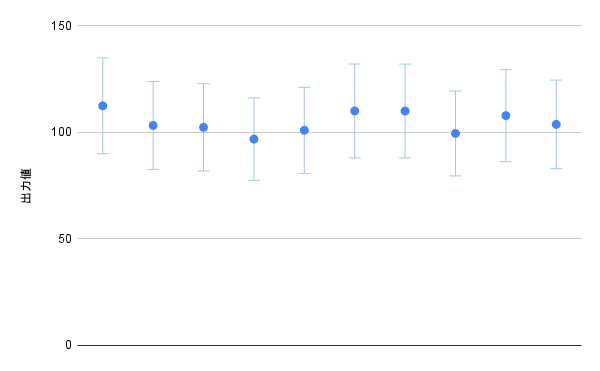
\includegraphics[height=80mm]{noise.png}
    \caption{差分プライバシーを適用した出力結果}
    \label{fig:noise}
\end{figure}

\subsection{計算時間の測定}

先ほどと同様に1000マイルを超えるタクシーの距離を利用したユーザーの数をカウントする処理を行った。
計算時間は、以下の4パターンで比較をした。
\begin{itemize}
    \item サンプルプログラムを機械語に直接コンパイルした場合
    \item サンプルプログラムをWebAssemblyにコンパイルしサンドボックスで動作させた場合
    \item サンプルプログラムをサンドボックス上で動作させ、何もノイズを付加しない門番を動作させた場合
    \item サンプルプログラムをサンドボックス上で動作させ、ノイズを付加する門番を動作させた場合
\end{itemize}

以上の実行結果を図\ref{fig:time}に示す。

サンプルプログラムを機械語に直接コンパイルした場合の平均実行時間が2.05499秒、
サンプルプログラムをWebAssemblyにコンパイルしサンドボックスで動作させた場合は2.94702秒、
サンプルプログラムをサンドボックス上で動作させ、何もノイズを付加しない門番を動作させた場合は2.98434秒、
サンプルプログラムをサンドボックス上で動作させ、ノイズを付加する門番を動作させた場合は2.96644秒となった。
これを倍率に直すと、直接コンパイルしたものを1として、それぞれ1.434079971、1.452240644、1.443530139となる。
この結果から、本実験ではオーバーヘッドとして約1.44倍の計算時間が発生していることがわかる。

\begin{figure}[htbp]
    \centering
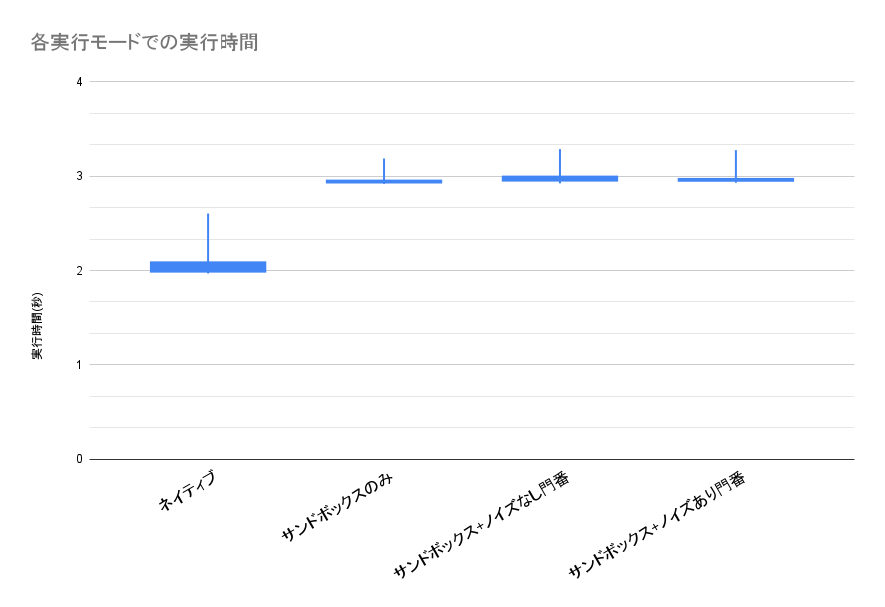
\includegraphics[height=100mm]{time.png}
    \caption{各種条件下での実行時間の比較}
    \label{fig:time}
\end{figure}

\chapter{応用}

\subsection{複数の言語での実装}

本研究では実験プログラムをRust言語を用いて開発した。ランタイムがRust言語で開発されていたためコードの
相互利用性を高めるのが理由である。しかし冒頭で示したようにWebAssemblyはターゲットとして対応するプログラム言語の
コンパイラから出力できるため、C言語やgo言語など複数の言語に対応できる。
応用例としては既存の別言語で書かれたプログラムを、言語仕様を変えないままWebAssemblyに変換し
WASI対応のバイナリーとして差分プライバシーを適用することが考えられる。

\chapter{課題}

\section{出力誤差について}

差分プライバシーでの出力比較実験で示したように、本システムでは繰り返し同じ統計計算を行うことで、真の値に近しい統計値へ
ノイズ込みの出力を近似できる。しかし、実運用ではこの挙動は攻撃者に真の値を決定させる情報を与えることになるため好ましくない。
これに対応する策としては、何らかのバジェット(予算)を各プログラムに設定し、同じ統計値を繰り返し求める場合の回数制限を
導入するような改良が必要になると考えられる。

\section{オーバーヘッドについて}

計算時間の測定実験で示したように、現状門番の差分プライバシーを適用した場合にオーバーヘッドが発生している。
またWebAssemblyとして動作させる場合に、アーキテクチャによっては他の言語で書かれたネイティブプログラムよりも遅くなることがある。
これらの2つのオーバーヘッドは課題としてあげられる。

\chapter{結論}
本研究では、差分プライバシーを適用しながらも複雑な統計処理を実現するための新たな手法を提案した。
それだけではなく、提案手法を実装し提案システム通り差分プライバシーが動作していることを確認した。
また性能を評価し、オーバーヘッドが大幅に大きく式を立てることができる。
本実装により、個人情報を含むデータに対するプライバシー保護を実現できるだけでなく、
新たに複雑な統計処理が実現可能となった。
ただし、ノイズの予算や大きさなど実利用のためには調整しないといけない点が多いことは今後の課題である。

\chapter*{謝辞}
\addcontentsline{toc}{chapter}{\numberline{}謝辞}

% textlint-disable preset-ja-technical-writing/no-mix-dearu-desumasu

本研究の提案から遂行、論文執筆など多岐に渡り、指導教員として筑波大学の建部先生、東京大学の田浦先生に多大なるご指導を賜りました。
深く感謝いたします。
また研究や実装にあたりHPCS研究室の皆様にご助言とご支援いただきました。
ここに感謝の意を表します。
最後に、本実装の中で使用したオープンソースソフトウェア・ライブラリ・エコシステム等の開発者の皆様にもお礼申し上げます。

% textlint-enable preset-ja-technical-writing/no-mix-dearu-desumasu

\newpage

\addcontentsline{toc}{chapter}{\numberline{}参考文献}
\renewcommand{\bibname}{参考文献}

%\bibliographystyle{junsrt}
%\bibliography{samplebib}
%% [compile] jbibtex sample; platex sample; platex sample;

% textlint-disable ja-engineering-paper/unify-kuten-and-touten
\begin{thebibliography}{1}
    \bibitem{dpsql}
    Royce J. Wilson and
    Celia Yuxin Zhang and
    William Lam and
    Damien Desfontaines and
    Daniel Simmons-Marengo and
    Bryant Gipson.
    \newblock Differentially Private SQL with Bounded User Contribution.

    \bibitem{dp}
    寺田 雅之
    \newblock  差分プライバシーとは何か, システム/制御/情報, 2019, 63 巻, 2 号, p. 58-63, 公開日 2019/08/15, Online ISSN 2424-1806, Print ISSN 0916-1600

    \bibitem{dp2}
    Cynthia Dwork, "Differential Privacy"

    \bibitem{googledp}
    https://github.com/google/differential-privacy

    \bibitem{openmind}
    https://github.com/OpenMined/PipelineDP

    \bibitem{apple}
    \newblock https://www.apple.com/privacy/docs/Differential\_Privacy\_Overview.pdf

    \bibitem{rand}
    あつまれ統計の森
    \newblock 逆関数法 -任意の確率分布に従う乱数を生成する
     - https://www.hello-statisticians.com/explain-terms-cat/inverse-transformation-method.html

    \bibitem{wasmtime}
    https://github.com/bytecodealliance/wasmtime

    \bibitem{wasmer}
    https://github.com/wasmerio/wasmer

    \bibitem{wasi}
    https://github.com/WebAssembly/WASI

    \bibitem{k-anon}
    村本俊祐; 上土井陽子; 若林真一. k-匿名性を利用したデータ一般化によるプライバシー保護. DEWS2007, 2007.

    \bibitem{apache}
    https://spark.apache.org/

    \bibitem{wasi-pr-thread}
    https://github.com/WebAssembly/wasi-libc/pull/311

    \bibitem{wasi-issue-thread}
    https://github.com/WebAssembly/wasi-libc/issues/209

\end{thebibliography}
% textlint-enable ja-engineering-paper/unify-kuten-and-touten

%%\begin{thebibliography}{1}
%%\bibitem{Bibunsho}
%%奥村 晴彦, 黒木 裕介.
%%\newblock LaTeX2ε美文書作成入門 改訂第7版.
%%\newblock 技術評論社, 2017.
%%
%%\bibitem{ScienceResearchWriting}
%%Hilary Glasman-Deal.
%%\newblock Science Research Writing: A Guide for Non-Native Speakers of English.
%%\newblock Imperial College Press, 2009.
%%\end{thebibliography}

\end{document}
